\documentclass{standalone}
\usepackage{tikz}
\usetikzlibrary{patterns, positioning}


\begin{document}
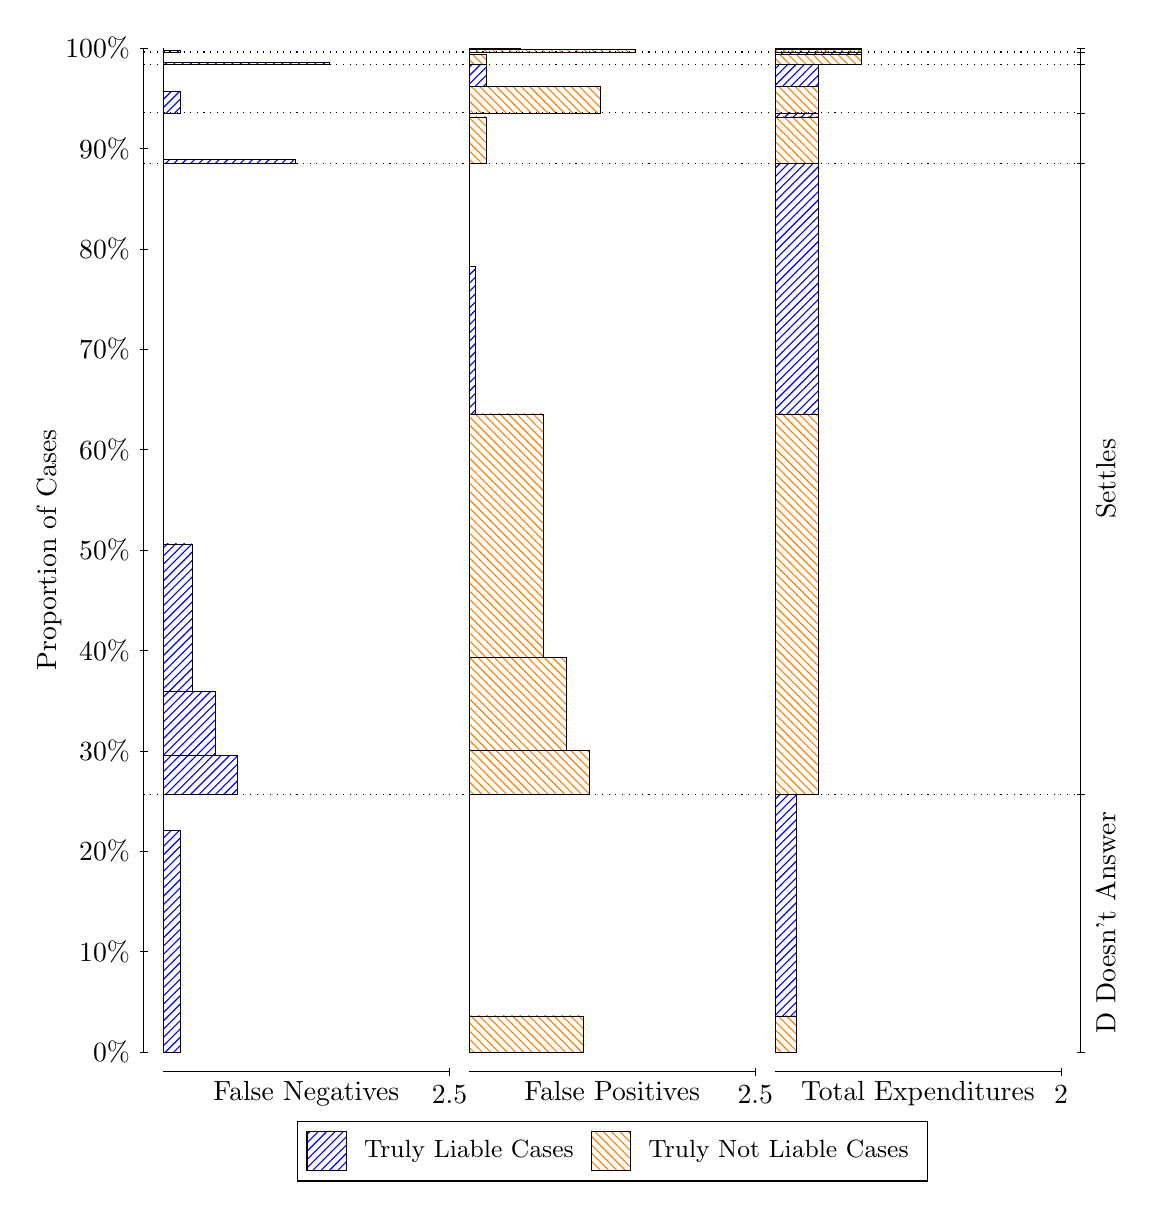
\begin{tikzpicture}
\draw[black, very thin] (1.5,1.75) -- (1.5,14.5);
\node[rotate=90, text=black, anchor=center] at (0.3, 8.125) {Proportion of Cases};
\draw[black, very thin] (1.45,1.75) -- (1.55,1.75);
\node[text=black, anchor=east] at (1.45, 1.75) {0\%};
\draw[black, very thin] (1.45,3.025) -- (1.55,3.025);
\node[text=black, anchor=east] at (1.45, 3.025) {10\%};
\draw[black, very thin] (1.45,4.3) -- (1.55,4.3);
\node[text=black, anchor=east] at (1.45, 4.3) {20\%};
\draw[black, very thin] (1.45,5.575) -- (1.55,5.575);
\node[text=black, anchor=east] at (1.45, 5.575) {30\%};
\draw[black, very thin] (1.45,6.85) -- (1.55,6.85);
\node[text=black, anchor=east] at (1.45, 6.85) {40\%};
\draw[black, very thin] (1.45,8.125) -- (1.55,8.125);
\node[text=black, anchor=east] at (1.45, 8.125) {50\%};
\draw[black, very thin] (1.45,9.4) -- (1.55,9.4);
\node[text=black, anchor=east] at (1.45, 9.4) {60\%};
\draw[black, very thin] (1.45,10.675) -- (1.55,10.675);
\node[text=black, anchor=east] at (1.45, 10.675) {70\%};
\draw[black, very thin] (1.45,11.95) -- (1.55,11.95);
\node[text=black, anchor=east] at (1.45, 11.95) {80\%};
\draw[black, very thin] (1.45,13.225) -- (1.55,13.225);
\node[text=black, anchor=east] at (1.45, 13.225) {90\%};
\draw[black, very thin] (1.45,14.5) -- (1.55,14.5);
\node[text=black, anchor=east] at (1.45, 14.5) {100\%};

\draw[black, very thin] (13.4,1.75) -- (13.4,14.5);
\draw[black, very thin] (13.35,1.75) -- (13.45,1.75);
\node[anchor=west] at (13.35, 1.75) {};
\draw[black, very thin] (13.35,5.0249) -- (13.45,5.0249);
\node[anchor=west] at (13.35, 5.0249) {};
\draw[black, very thin] (13.35,13.031) -- (13.45,13.031);
\node[anchor=west] at (13.35, 13.031) {};
\draw[black, very thin] (13.35,13.677) -- (13.45,13.677);
\node[anchor=west] at (13.35, 13.677) {};
\draw[black, very thin] (13.35,14.291) -- (13.45,14.291);
\node[anchor=west] at (13.35, 14.291) {};
\draw[black, very thin] (13.35,14.45) -- (13.45,14.45);
\node[anchor=west] at (13.35, 14.45) {};
\draw[black, very thin] (13.35,14.5) -- (13.45,14.5);
\node[anchor=west] at (13.35, 14.5) {};

\draw[black, very thin, pattern color=blue, pattern=north east lines] (1.75,1.75) rectangle (1.968,4.567);
\draw[black, very thin, pattern color=orange, pattern=north west lines] (1.75,4.567) rectangle (1.75,5.0249);
\draw[black, very thin, pattern color=blue, pattern=north east lines] (1.75,5.0249) rectangle (2.6947,5.5137);
\draw[black, very thin, pattern color=blue, pattern=north east lines] (1.75,5.5137) rectangle (2.404,6.3333);
\draw[black, very thin, pattern color=blue, pattern=north east lines] (1.75,6.3333) rectangle (2.1133,8.2035);
\draw[black, very thin, pattern color=orange, pattern=north west lines] (1.75,8.2035) rectangle (1.75,13.031);
\draw[black, very thin, pattern color=blue, pattern=north east lines] (1.75,13.031) rectangle (3.4213,13.083);
\draw[black, very thin, pattern color=orange, pattern=north west lines] (1.75,13.083) rectangle (1.75,13.677);
\draw[black, very thin, pattern color=blue, pattern=north east lines] (1.75,13.677) rectangle (1.968,13.954);
\draw[black, very thin, pattern color=orange, pattern=north west lines] (1.75,13.954) rectangle (1.75,14.291);
\draw[black, very thin, pattern color=blue, pattern=north east lines] (1.75,14.291) rectangle (3.8573,14.319);
\draw[black, very thin, pattern color=orange, pattern=north west lines] (1.75,14.319) rectangle (1.75,14.45);
\draw[black, very thin, pattern color=blue, pattern=north east lines] (1.75,14.45) rectangle (1.968,14.472);
\draw[black, very thin, pattern color=orange, pattern=north west lines] (1.75,14.472) rectangle (1.75,14.5);
\draw[black, very thin, pattern color=orange, pattern=north west lines] (5.6333,1.75) rectangle (7.0867,2.2079);
\draw[black, very thin, pattern color=blue, pattern=north east lines] (5.6333,2.2079) rectangle (5.6333,5.0249);
\draw[black, very thin, pattern color=orange, pattern=north west lines] (5.6333,5.0249) rectangle (7.1593,5.5778);
\draw[black, very thin, pattern color=orange, pattern=north west lines] (5.6333,5.5778) rectangle (6.8687,6.7575);
\draw[black, very thin, pattern color=orange, pattern=north west lines] (5.6333,6.7575) rectangle (6.578,9.8525);
\draw[black, very thin, pattern color=blue, pattern=north east lines] (5.6333,9.8525) rectangle (5.706,11.723);
\draw[black, very thin, pattern color=blue, pattern=north east lines] (5.6333,11.723) rectangle (5.6333,13.031);
\draw[black, very thin, pattern color=orange, pattern=north west lines] (5.6333,13.031) rectangle (5.8513,13.625);
\draw[black, very thin, pattern color=blue, pattern=north east lines] (5.6333,13.625) rectangle (5.6333,13.677);
\draw[black, very thin, pattern color=orange, pattern=north west lines] (5.6333,13.677) rectangle (7.3047,14.014);
\draw[black, very thin, pattern color=blue, pattern=north east lines] (5.6333,14.014) rectangle (5.8513,14.291);
\draw[black, very thin, pattern color=orange, pattern=north west lines] (5.6333,14.291) rectangle (5.8513,14.421);
\draw[black, very thin, pattern color=blue, pattern=north east lines] (5.6333,14.421) rectangle (5.6333,14.45);
\draw[black, very thin, pattern color=orange, pattern=north west lines] (5.6333,14.45) rectangle (7.7407,14.478);
\draw[black, very thin, pattern color=blue, pattern=north east lines] (5.6333,14.478) rectangle (6.2873,14.5);
\draw[black, very thin, pattern color=orange, pattern=north west lines] (9.5167,1.75) rectangle (9.7892,2.2079);
\draw[black, very thin, pattern color=blue, pattern=north east lines] (9.5167,2.2079) rectangle (9.7892,5.0249);
\draw[black, very thin, pattern color=orange, pattern=north west lines] (9.5167,5.0249) rectangle (10.062,9.8525);
\draw[black, very thin, pattern color=blue, pattern=north east lines] (9.5167,9.8525) rectangle (10.062,13.031);
\draw[black, very thin, pattern color=orange, pattern=north west lines] (9.5167,13.031) rectangle (10.062,13.625);
\draw[black, very thin, pattern color=blue, pattern=north east lines] (9.5167,13.625) rectangle (10.062,13.677);
\draw[black, very thin, pattern color=orange, pattern=north west lines] (9.5167,13.677) rectangle (10.062,14.014);
\draw[black, very thin, pattern color=blue, pattern=north east lines] (9.5167,14.014) rectangle (10.062,14.291);
\draw[black, very thin, pattern color=orange, pattern=north west lines] (9.5167,14.291) rectangle (10.607,14.421);
\draw[black, very thin, pattern color=blue, pattern=north east lines] (9.5167,14.421) rectangle (10.607,14.45);
\draw[black, very thin, pattern color=orange, pattern=north west lines] (9.5167,14.45) rectangle (10.607,14.478);
\draw[black, very thin, pattern color=blue, pattern=north east lines] (9.5167,14.478) rectangle (10.607,14.5);
\draw[black, dotted] (1.5,5.0249) -- (13.4,5.0249);
\draw[black, dotted] (1.5,13.031) -- (13.4,13.031);
\draw[black, dotted] (1.5,13.677) -- (13.4,13.677);
\draw[black, dotted] (1.5,14.291) -- (13.4,14.291);
\draw[black, dotted] (1.5,14.45) -- (13.4,14.45);
\draw[black, very thin] (1.75,1.5) -- (5.3833,1.5);
\node[text=black, anchor=north] at (3.5667, 1.5) {False Negatives};
\draw[black, very thin] (5.3833,1.45) -- (5.3833,1.55);
\node[text=black, anchor=north] at (5.3833, 1.45) {2.5};

\draw[black, very thin] (5.6333,1.5) -- (9.2667,1.5);
\node[text=black, anchor=north] at (7.45, 1.5) {False Positives};
\draw[black, very thin] (9.2667,1.45) -- (9.2667,1.55);
\node[text=black, anchor=north] at (9.2667, 1.45) {2.5};

\draw[black, very thin] (9.5167,1.5) -- (13.15,1.5);
\node[text=black, anchor=north] at (11.333, 1.5) {Total Expenditures};
\draw[black, very thin] (13.15,1.45) -- (13.15,1.55);
\node[text=black, anchor=north] at (13.15, 1.45) {2};

\node[text=black, centered, rotate=90] at (13.72, 3.3874) {D Doesn't Answer};
\node[text=black, centered, rotate=90] at (13.72, 9.028) {Settles};





\draw (7.449999999999999,1.5) node[draw=none] (baseCoordinate) {};
\begin{scope}[align=center]
        \matrix[scale=0.5, draw=black, below=0.5cm of baseCoordinate, nodes={draw}, column sep=0.1cm]{
            \node[rectangle, draw, minimum width=0.5cm, minimum height=0.5cm, pattern color=blue, pattern=north east lines] {}; &
            \node[draw=none, font=\small, text=black] (B) {Truly Liable Cases}; &
            \node[rectangle, draw, minimum width=0.5cm, minimum height=0.5cm, pattern color=orange, pattern=north west lines] {}; &
            \node[draw=none, font=\small, text=black] (B) {Truly Not Liable Cases}; \\
            };
\end{scope}

\end{tikzpicture}
\end{document}